\subsection{测度的支集}

设 \(\mu\) 是局部紧空间 \(X\) 上的一个测度，设 \(\mathfrak{G}\) 是开集 \(U \subset X\) （\(\mu\) 在 \(U\) 上的限制为零）所成的集；由局部化原理（No.~1, 命题 1 的推论）立即可知，若 \(U_0\) 是诸集 \(U \in \mathfrak{G}\) 的并，则 \(U_0\) 本身属于 \(\mathfrak{G}\) ，因而是 \(\mathfrak{G}\) 中最大的开集。

定义 1. --- 设 \(\mu\) 是局部紧空间 \(X\) 上的一个测度，我们把 \(\mu\) 的支集（记作 \(\operatorname{Supp}(\mu)\) ）定义为 \(X\) 中使 \(\mu\) 的限制为零的最大开集的余闭集。

说一点 \(x \in X\) 不属于 \(\mu\) 的支集，意味着存在 x 的一个开邻域 V 使 \(\mu\) 在 V 上的限制为零；因此，说 x 属于 \(\mu\) 的支集，就意味着对 x 的每个邻域 V，存在一个函数 \(f \in \mathcal{K}(X; \mathbf{C})\) ，其支集含于 V，使 \(\mu(f) \neq 0\) 。

例子. --- 1) 为使 X 上的一个测度为零，必须且只须其支集为空集。

\begin{enumerate}
\def\labelenumi{\arabic{enumi})}
\setcounter{enumi}{1}
\item
  \(\mathbf{R}\) 上的 Lebesgue 测度的支集是整条直线 \(\mathbf{R}\) ；因为它是非空的，且在每个平移下不变。
\item
  在区间 \(\mathrm{X} = [0,1]\) （\(\mathbf{R}\) 中）上取一个可数稠密集，把它排成序列 \((a_n)\) ，并设 \(\mu\) 是把质量 \(2^{-n}\) 放在点 \(a_n\) 处（对每个 \(n \geqslant 0\) ）所定义的测度（§1, No.~3, 例 I）。 \(\mu\) 的支集是整个 \(\mathrm{X}\) ；因为设 \(x\) 是 \(\mathrm{X}\) 的任一点， \(\mathrm{V}\) 是 \(x\) 的一个邻域， \(f\) 是一个连续实值函数， \(\geqslant 0\) 于 \(\mathrm{X}\) ，在点 \(x\) 处等于 1，且其支集含于 \(\mathrm{V}\) （§1, No.~2, 引理 1）；\(y \in \mathrm{V}\) （\(f(y) > 0\) ）所成之集在 \(\mathrm{X}\) 中是开集，因而包含某点 \(a_n\) ，于是 \(\mu(f) \geqslant f(a_n)2^{-n} > 0\) 。
\end{enumerate}

命题 2. --- 测度 \(\mu\) 的支集与测度 \(|\mu|\) 的支集相同；若 \(\mu\) 是实测度，则其支集是测度 \(\mu^{+}\) 与 \(\mu^{-}\) 的支集之并。

因为若 \(\mu\) 在某个开集 U 上的限制为零，则 \(|\mu|\) 的限制（相应地， \(\mu^{+}\) 与 \(\mu^{-}\) 的限制，当 \(\mu\) 为实测度时）也为零，反之亦然。

\pandocbounded{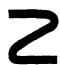
\includegraphics[keepaspectratio]{images/part001_dfbe8ad7.jpg}}

注意， \(\mu^{+}\) 与 \(\mu^{-}\) 的支集可以都非空且相同（参见 Ch. V, § 5, 习题 5）。

命题 3. --- 若 \(\mu\) 与 \(\nu\) 是局部紧空间 X 上满足 \(|\mu| \leqslant |\nu|\) 的两个测度，则 \(\operatorname{Supp}(\mu) \subset \operatorname{Supp}(\nu)\) 。

因为若 \(\nu\) 在某个开集上的限制为零，则 \(\mu\) 的限制也为零。

命题 4. --- 两个测度之和的支集含于其支集之并。

因为若两个测度在某个开集上的限制为零，则其和的限制同样为零。

若 \(\mu\) 与 \(\nu\) 是两个正测度，则 \(\lambda = \mu + \nu\) 的支集等于 \(\mu\) 与 \(\nu\) 的支集之并；因为若 \(x_0\) 是该并中的一点且 V 是 \(x_0\) 的任一邻域，则存在一个连续函数 \(f \geqslant 0\) ，其支集含于 V，且使 \(\mu(f)\) 、 \(\nu(f)\) 两数之一 \(>0\) ；更有甚者， \(\lambda(f) = \mu(f) + \nu(f) > 0\) 。

命题 5. --- 测度 \(\mu\) 在开集 U 上的限制的支集是 \(\mu\) 的支集在 U 上的迹。

由定义，该命题是显然的。

命题 6. --- 局部紧空间 X 上支集含于一个闭集 F 的测度所成之集，是 \(\mathcal{M}(\mathrm{X};\mathbf{C})\) 的一个淡闭线性子空间。

因为它是方程为 \(\mu(f) = 0\) 的淡闭超平面之交，其中 f 跑遍 \(\mathcal{K}(\mathrm{X};\mathbf{C})\) 中支集与 F 不相交的函数所成之集。

设 X 不是紧的：给定一个滤子 \(\Phi\) （在 X 上测度的空间 \(\mathcal{M}(\mathrm{X};\mathbf{C})\) 上），我们说测度 \(\mu\) 的支集沿 \(\Phi\) 退向无穷，如果对 X 的每个紧子集 K，存在一个集 \(M\in\Phi\) ，使得 \(\operatorname{Supp}(\mu)\cap K=\varnothing\) 对每个测度 \(\mu\in M\) 成立。

命题 7. --- 若 \(\Phi\) 是 \(\mathcal{M}(\mathrm{X};\mathbf{C})\) 上的一个滤子，使得测度 \(\mu\) 的支集沿 \(\Phi\) 退向无穷，则 \(\mu\) 关于 \(\Phi\) 淡收敛于 0。

设 \(f\) 是 \(\mathcal{K}(\mathrm{X};\mathbf{C})\) 中的任一函数， \(K\) 是其支集。按假设，存在一个集 \(M \in \Phi\) ，使得对每个测度 \(\mu \in M\) ， \(\operatorname{Supp}(\mu) \cap K = \varnothing\) ；由此得 \(\mu(f) = 0\) 对所有 \(\mu \in M\) 成立，这就证明了该命题。

